\documentclass[a4paper]{article}
\usepackage{vntex}
\usepackage{a4wide,amssymb,epsfig,latexsym,array,hhline,fancyhdr}
\usepackage{amsmath}
\usepackage{amsthm}
\usepackage{multicol,longtable,amscd}
\usepackage{diagbox}
\usepackage{booktabs}
\usepackage{alltt}
\usepackage[framemethod=tikz]{mdframed}
\usepackage{caption,subcaption}
\usepackage{lastpage}
\usepackage[lined,boxed,commentsnumbered]{algorithm2e}
\usepackage{enumerate}
\usepackage{color}
\usepackage{graphicx}
\usepackage{array}
\usepackage{tabularx, caption}
\usepackage{multirow}
\usepackage{multicol}
\usepackage{rotating}
\usepackage{graphics}
\usepackage{geometry}
\usepackage{setspace}
\usepackage{epsfig}
\usepackage{tikz}
\usepackage[british]{babel}

\usetikzlibrary{arrows,snakes,backgrounds}
\usepackage[unicode]{hyperref}
\usepackage{import}
\hypersetup{urlcolor=blue,linkcolor=black,citecolor=black,colorlinks=true}

\setlength{\headheight}{40pt}
\pagestyle{fancy}
\fancyhead{} % clear all header fields
\fancyhead[L]{
    \begin{tabular}{rl}
        \begin{picture}(25,15)(0,0)
            \put(0,-8){
\includegraphics[width=8mm, height=8mm]{image/local/hcmut.png}}
            %\put(0,-8){\epsfig{width=10mm,figure=hcmut.eps}}
        \end{picture} &
        %
\includegraphics[width=8mm, height=8mm]{hcmut.png} & %
        \begin{tabular}{l}
            \textbf{\bf \ttfamily Trường Đại Học Bách Khoa Tp.Hồ Chí Minh} \\
            \textbf{\bf \ttfamily Khoa Khoa Học và Kỹ Thuật Máy Tính}
        \end{tabular}
    \end{tabular}
}
\fancyhead[R]{
    \begin{tabular}{l}
        \tiny \bf \\
        \tiny \bf
    \end{tabular}  }
\fancyfoot{} % clear all footer fields
\fancyfoot[L]{\scriptsize \ttfamily GIAI ĐOẠN 1: ĐỀ CƯƠNG LUẬN VĂN/ ĐỒ ÁN CHUYÊN NGÀNH/
ĐỒ ÁN MÔN HỌC KỸ THUẬT MÁY TÍNH - HỌC KỲ 2 NĂM HỌC 2023-2024}
\fancyfoot[R]{\scriptsize \ttfamily Trang {\thepage}/\pageref{LastPage}}
\renewcommand{\headrulewidth}{0.3pt}
\renewcommand{\footrulewidth}{0.3pt}

\setcounter{secnumdepth}{4}
\setcounter{tocdepth}{3}
\makeatletter
\newcounter {subsubsubsection}[subsubsection]
\renewcommand\thesubsubsubsection{\thesubsubsection .\@alph\c@subsubsubsection}
\newcommand\subsubsubsection{\@startsection{subsubsubsection}{4}{\z@}%
{-3.25ex\@plus -1ex \@minus -.2ex}%
{1.5ex \@plus .2ex}%
{\normalfont\normalsize\bfseries}}
\newcommand*\l@subsubsubsection{\@dottedtocline{3}{10.0em}{4.1em}}
\newcommand*{\subsubsubsectionmark}[1]{}

\sloppy
\captionsetup[figure]{labelfont={small,bf},textfont={small,it},belowskip=0pt,aboveskip=0pt}
\captionsetup[table]{labelfont={small,bf},textfont={small,it},belowskip=-1pt,aboveskip=7pt}
\setlength{\floatsep}{5pt plus 2pt minus 2pt}
\setlength{\textfloatsep}{5pt plus 2pt minus 2pt}
\setlength{\intextsep}{10pt plus 2pt minus 2pt}

\begin{document}
%%%%%%%%%%%%%%%%%%%%%%%%%%%%%%%%%%%%%%%%%%%%%%%%%%%%%%%%%%%%%%%%%%%
    \begin{titlepage}
    \begin{center}
        ĐẠI HỌC QUỐC GIA THÀNH PHỐ HỒ CHÍ MINH \\
        TRƯỜNG ĐẠI HỌC BÁCH KHOA \\
        KHOA KHOA HỌC - KỸ THUẬT MÁY TÍNH
    \end{center}
    \vspace{1cm}
    \begin{figure}[h!]
        \begin{center}
            
\includegraphics[width=4cm]{image/local/hcmut}
        \end{center}\label{fig:figure}
    \end{figure}
    \vspace{1cm}
    \begin{center}
        \begin{tabular}{c}
            \multicolumn{1}{l}{\textbf{{\Large GIAI ĐOẠN 1 (GĐ1):}}}                                       \\
            \multicolumn{1}{l}{\textbf{{ĐỀ CƯƠNG LUẬN VĂN/ ĐỒ ÁN CHUYÊN NGÀNH/}}}                          \\
            \multicolumn{1}{l}{\textbf{{ĐỒ ÁN MÔN HỌC KỸ THUẬT MÁY TÍNH}}}                                 \\
            ~~                                                                                             \\
            \hline
            \\
            \multicolumn{1}{l}{\textbf{{\Large Tên đề tài}}}\\
            \multicolumn{1}{l}{\textbf{{Tiếng Việt: Rút trích quan hệ giữa Ý định và Thực thể}}}                            \\
            \multicolumn{1}{l}{\textbf{{ sử dụng hướng tiếp cận Đọc hiểu Máy}}}\\
            \multicolumn{1}{l}{\textbf{{ cho nhiệm vụ xây dựng Đồ thị Tri thức trong lĩnh vực Giáo dục.}}}                          \\
            \\
            \multicolumn{1}{l}{\textbf{{Tiếng Anh: Relation Extraction between}}}\\
            \multicolumn{1}{l}{\textbf{{ Intent and Entity using Machine Reading Comprehension(MRC)}}}\\
            \multicolumn{1}{l}{\textbf{{ approach for Knowledge}}}\\
            \multicolumn{1}{l}{\textbf{{ Graph Construction in Education domain.}}}\\


            \\
            \hline
        \end{tabular}
    \end{center}

    \vspace{0.7cm}

    \begin{table}[h]
        \centering \large
        \begin{tabular}{rll}
            \textbf{Giáo viên hướng dẫn 1:} & Bùi Công Tuấn &         \\
            \textbf{Giáo viên hướng dẫn 2:} & Bùi Công Tuấn &         \\
            \textbf{SV thực hiện:}        & Lưu Quốc Bình & 2033009 \\
        \end{tabular}\label{tab:table}
    \end{table}

    \vspace{1.0cm}
    \begin{center}
    {\footnotesize Tp. Hồ Chí Minh, Tháng 05 Năm 2024}
    \end{center}
\end{titlepage}

    \newpage
    \tableofcontents
%%%%%%%%%%%%%%%%%%%%%%%%%%%%%%%%%%%%%%%%%%%%%%%%%%%%%%%%%%%%%%%%%%%
    \newpage
    \section{Giới thiệu}\label{sec:gioi-thieu}
%%%%%%%%%%%%%%%%%%%%%%%%%%%%%%%%%%%%%%%%%%%%%%%%%%%%%%%%%%%%%%%%%%%
    \newpage
    \section{Phương pháp trích xuất quan hệ}\label{sec:phuong-phap-trich-xuat-quan-he}

\subsection{Các phương pháp truyền thống}\label{subsec:cac-phuong-phap-truyen-thong}

\begin{singlespace}
    Như được thể hiện trong Hình 1,
    các phương pháp trích xuất quan hệ (RE) hiện có có thể được phân loại thành hai loại chính:
    Phương pháp truyền thống (\underline{Traditional Methods}) và Phương pháp học sâu (\underline{Deep Learning Methods}).
    Phương pháp truyền thống sử dụng các kỹ thuật dựa trên luật (\underline{Rule Based Methods}) hoặc kỹ thuật học máy để trích xuất một tập hợp các quan hệ được xác định trước từ một kho văn bản (corpus).
    Các phương pháp truyền thống có thể được phân loại chi tiết thành phương pháp dựa trên luật (\underline{Rule Based Methods}) và phương pháp học máy (\underline{Machine Learning Methods}).
\end{singlespace}

\begin{singlespace}
    Các phương pháp học máy (\underline{Machine Learning Methods}) có thể được phân loại thêm thành bốn loại:
    (1) Phương pháp không giám sát (Unsupervised Learning Methods).
    (2) Phương pháp có giám sát (Supervised Learning Methods).
    (3) Phương pháp bán giám sát (Semi-supervised).
    và (4) Phương pháp Giám sát từ xa (Distant supervision).
\end{singlespace}

\begin{figure}[h!]
    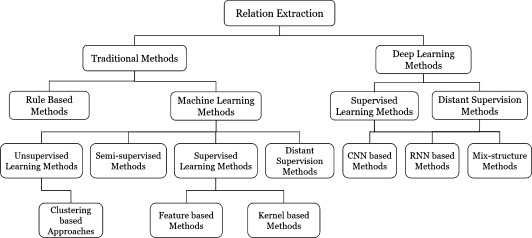
\includegraphics
    [width=0.9\textwidth]{image/parts/1}
    \begin{center}
        \begin{tablenotes}
            \item{Nguồn: https://www.sciencedirect.com/science/article/pii/S2667305323000698#br0060}
        \end{tablenotes}
    \end{center}
    \renewcommand{\figurename}{Hình.}
    \caption{Các loại phương pháp trích xuất quan hệ.}\label{fig:image/parts/1}
\end{figure}

\begin{itemize}
    \item Phương pháp dựa trên luật ({Rule-based}): Sử dụng các quy tắc thủ công được thiết lập sẵn để trích xuất quan hệ.
    \item Phương pháp không giám sát (Unsupervised): Tự động học các mẫu trích xuất quan hệ từ dữ liệu.
    \item Phương pháp có giám sát (Supervised): Sử dụng dữ liệu được dán nhãn để huấn luyện mô hình trích xuất quan hệ.
    \item Phương pháp bán giám sát (Semi-supervised): Kết hợp dữ liệu được dán nhãn và không được dán nhãn để huấn luyện mô hình.
    \item Phương pháp giám sát từ xa (Distant supervision): Sử dụng dữ liệu gián tiếp để huấn luyện mô hình.
\end{itemize}

\subsubsection{Phương pháp dựa trên luật ({Rule-based})}
Các phương pháp này còn được gọi là phương pháp mẫu thủ công (hand-built pattern methods).
Chúng xác định một tập hợp các mẫu trích xuất (\href{https://www.sciencedirect.com/topics/computer-science/extraction-pattern}{extraction patterns}) cho các quan hệ được định nghĩa trước.
Sau đó, các mẫu trích xuất này được đối chiếu với văn bản. Nếu một mẫu khớp với văn bản, thì một quan hệ tương ứng với
mẫu đó được tìm thấy trong văn bản.
\href{https://www.scopus.com/record/display.uri?eid=2-s2.0-0027709268&origin=inward&txGid=dd620e007b93bb0bb26ec41071050554}{Riloff (1993)},
\href{https://scholar.google.com/scholar_lookup?title=Fastus%3A%20A%20finite-state%20processor%20for%20information%20extraction%20from%20real-world%20text&publication_year=1993&author=D.%20Appelt&author=J.%20Hobbs&author=J.%20Bear&author=D.%20Israel&author=M.%20Tyson}{Appelt et al. (1993)},
\href{https://scholar.google.com/scholar_lookup?title=Snowball%3A%20Extracting%20relations%20from%20large%20plain-text%20collections&publication_year=2000&author=E.%20Agichtein&author=L.%20Gravano}{Agichtein và Gravano (2000)},
\href{https://scholar.google.com/scholar_lookup?title=Avatar%20information%20extraction%20system&publication_year=2006&author=T.%20Jayram&author=R.%20Krishnamurthy&author=S.%20Raghavan&author=S.%20Vaithyanathan&author=H.%20Zhu}{Jayram et al. (2006)},
\href{https://www.scopus.com/inward/record.url?eid=2-s2.0-77951560898&partnerID=10&rel=R3.0.0}{Shen et al. (2007)},
\href{https://scholar.google.com/scholar_lookup?title=RelEx%20relation%20extraction%20using%20dependency%20parse%20trees&publication_year=2006&author=K.%20Fundel&author=R.%20K%C3%BCffner&author=R.%20Zimmer}{Fundel et al. (2006)},
\href{https://scholar.google.com/scholar_lookup?title=A%20rule-based%20relation%20extraction%20system%20using%20dbpedia%20and%20syntactic%20parsing&publication_year=2013&author=K.%20Nebhi}{Nebhi (2013)} đã sử dụng các phương pháp dựa trên luật để trích xuất quan hệ từ văn bản.
Bảng 3 hiển thị các ví dụ về quy tắc để trích xuất quan hệ hạ đẳng (hyponymy) từ văn bản.


%\begin{tabularx}{\textwidth}{p{5cm}|p{5cm}|p{5cm}|}
%\hline
%Pattern & Input sentence & Extracted relations \\
%\hline
%such NP as & \ldots works by such authors as Herrick, Goldsmith, and Shakespeare.
%& Hyponym (“author”, “Herrick”),  Hyponym (“author”, “Goldsmith”),  Hyponym (“author”, “Shakespeare”)
%\hline
%NP {, NP}{,} & Bruises, wounds, broken bones or  other injuries\ldots
%& Hyponym (“bruise”, “injury”),  Hyponym (“wound”, “injury”),  Hyponym (“broken bones”, “injury”)
%\hline
%\end{tabularx}

\begin{figure}[h!]
    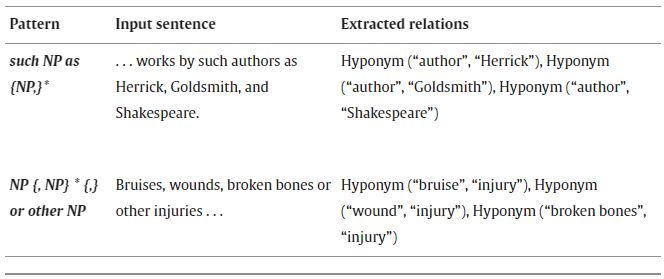
\includegraphics
    [width=0.9\textwidth]{image/parts/2}
    \begin{center}
        \begin{tablenotes}
        \end{tablenotes}
    \end{center}
    \renewcommand{\figurename}{Hình.}
    \caption{Ví dụ cho partern (mẫu/luật) Hyponyms (\href{https://www.sciencedirect.com/science/article/pii/S2667305323000698#br0500}{Hearst (1992)}).}\label{fig:image/parts/2}
\end{figure}

Các phương pháp dựa trên luật đòi hỏi chuyên môn về lĩnh vực và kiến thức ngôn ngữ để xác định các mẫu trích xuất.
Những phương pháp này phụ thuộc vào từng lĩnh vực cụ thể, trong đó cấu trúc của tài liệu là cố định và các quan hệ mục
tiêu được xác định trước. Nếu chuyển từ lĩnh vực này sang lĩnh vực khác, thì cần phải xác định lại một tập hợp mới các
quan hệ mục tiêu và mẫu trích xuất. Do đó, các phương pháp dựa trên luật đòi hỏi nhiều công sức thủ công và không thể sử
dụng cho các tập văn bản đa dạng (heterogeneous corpora).


\newpage

\subsubsection{Phương pháp không giám sát (Unsupervised)}
Phương pháp không giám sát không yêu cầu bất kỳ dữ liệu được dán nhãn nào. Hầu hết các phương pháp RE không giám sát sử
dụng cách tiếp cận dựa trên cụm (clustering). Một trong những phương pháp RE không giám sát dựa trên cụm tiên phong
được đề xuất bởi
\href{https://www.sciencedirect.com/science/article/pii/S2667305323000698#br0470}{Hasegawa et al. (2004)}. Họ sử dụng công cụ đánh nhãn Thực thể Danh riêng (NE) để trích xuất các thực
thể, cho phép tập trung chỉ vào các quan hệ với những thực thể được đề cập. Hình 2 minh họa các bước của phương pháp
học không giám sát:
\begin{itemize}
    \item (1) Nhận dạng các thực thể tên riêng trong kho văn bản.
    \item (2) Xác định các thực thể tên riêng đồng xuất hiện và ngữ cảnh của chúng.
    \item (3) Cụm các cặp thực thể dựa trên tính tương đồng ngữ cảnh.
    \item (4) Gán tên quan hệ ngữ nghĩa cho mỗi cụm.
\end{itemize}

\begin{figure}[h!]
    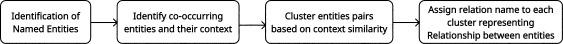
\includegraphics
    [width=0.9\textwidth]{image/parts/3}
    \begin{center}
        \begin{tablenotes}
        \end{tablenotes}
    \end{center}
    \renewcommand{\figurename}{Hình.}
    \caption{Cách tiếp cận dựa trên phân cụm cho \href{https://www.sciencedirect.com/topics/computer-science/unsupervised-learning}{Unsupervised Learning}.}\label{fig:figure2}
\end{figure}


\subsubsection{Phương pháp có giám sát (Supervised)}
Phương pháp có giám sát yêu cầu một lượng lớn dữ liệu huấn luyện được dán nhãn với tập hợp các thực thể và quan hệ. Phương pháp này sử dụng dữ liệu huấn luyện để đào tạo bộ phân loại, trích xuất quan hệ từ dữ liệu kiểm tra. Có hai loại phương pháp có giám sát: Phương pháp dựa trên đặc trưng (Feature-based methods) và Phương pháp dựa trên Hạt nhân (Kernel-based methods) (Pawar et al. (2017)).
\begin{itemize}
    \item
        Trong phương pháp dựa trên đặc trưng (Rink và Harabagiu (2010), Kambhatla (2004), Zhou et al. (2005)),
        một tập hợp các đặc trưng được tạo ra cho mỗi quan hệ trong dữ liệu huấn luyện, và bộ phân loại được đào
        tạo để trích xuất một thể hiện quan hệ mới. Một số đặc trưng về từ vựng (lexical), cú pháp (syntactic)
        và ngữ nghĩa (semantic) được mô tả trong (Kambhatla (2004)). Việc lựa chọn các đặc trưng ảnh hưởng đến hiệu
        suất của hệ thống RE có giám sát dựa trên đặc trưng.
    \item
        Không giống như phương pháp dựa trên đặc trưng, phương pháp dựa trên hàm nhân (Bunescu và Mooney, 2005b,
        Bunescu và Mooney, 2005a, Zelenko et al. (2003), Culotta và Sorensen (2004), Zhang et al. (2008),
        Zhang (2004)) không sử dụng các bước tiền xử lý để thiết kế đặc trưng. Trong phương pháp dựa trên hàm nhân,
        các \href{https://www.sciencedirect.com/topics/computer-science/kernel-function}{kernel functions} được sử dụng để xác định độ tương đồng giữa hai biểu diễn thể hiện quan hệ, trong khi Máy vectơ
        hỗ trợ (SVM) được sử dụng để phân loại. Hiệu suất của hệ thống RE dựa trên \href{https://www.sciencedirect.com/topics/computer-science/kernel-function}{kernel functions} phụ thuộc vào việc thiết
        kế các hàm nhân.

\end{itemize}

\subsubsection{Phương pháp bán giám sát (Semi-supervised)}
Việc tạo dữ liệu cho các phương pháp RE có giám sát đòi hỏi nhiều chi phí, nhân công và thời gian. Phương pháp bán giám
sát tự động tạo dữ liệu được dán nhãn bằng thuật toán bootstrapping. Cách tiếp cận này có hai ưu điểm: (1) giảm thiểu
công sức cần thiết để tạo dữ liệu được dán nhãn; (2) tận dụng dữ liệu không được dán nhãn \href{https://www.sciencedirect.com/topics/computer-science/unlabeled-data}{unlabeled data} sẵn có miễn phí.
Thuật toán bootstrapping yêu cầu một lượng lớn dữ liệu không được dán nhãn và một số ít instance hạt giống
(seed instance) của kiểu quan hệ mong muốn. Ví dụ, để trích xuất quan hệ "Thủ đô của" (CapitalOf), các instance
hạt giống "(New Delhi, Ấn Độ)", "(Canberra, Úc) và (London, Anh)" có thể được sử dụng để học một mẫu trích xuất.
Với các instance hạt giống này làm đầu vào, thuật toán bootstrapping có thể trích xuất các quan hệ tương tự với
các cặp thực thể như "(Paris, Pháp)".
\href{https://www.sciencedirect.com/science/article/pii/S2667305323000698#fg0030}{Hình 3} minh họa mô hình để
trích xuất các mẫu và các cặp thực thể hạt giống bằng phương pháp học bán giám sát.
KnowItAll (\href{https://www.sciencedirect.com/science/article/pii/S2667305323000698#br0340}{Etzioni et al. (2004)}),
TextRunner (\href{https://www.sciencedirect.com/science/article/pii/S2667305323000698#br0090}{Banko et al. (2007)}),
OLLIE (\href{https://www.sciencedirect.com/science/article/pii/S2667305323000698#br0820}{Mausam et al. (2012)}), v.v.
sử dụng phương pháp bán giám sát cho RE.

\begin{figure}[h!]
    \centering
    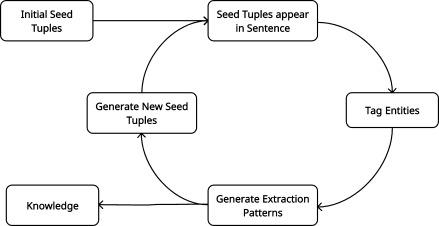
\includegraphics
    [width=0.8\textwidth]{image/parts/4}
    \begin{center}
        \begin{tablenotes}
        \end{tablenotes}
    \end{center}
    \renewcommand{\figurename}{Hình.}
    \caption{Phương pháp học bán giám sát (Semi-Supervised Learning) để trích xuất quan hệ.}\label{fig:figure3}
\end{figure}

\newpage
\subsubsection{Phương pháp giám sát từ xa (Distant supervision)}
Phương pháp này còn được gọi là phương pháp giám sát yếu (weakly supervised methods) hoặc phương pháp dựa trên
kiến thức (knowledge based methods).
\href{https://www.sciencedirect.com/science/article/pii/S2667305323000698#br0890}{Mintz et al. (2009)}
đã đề xuất phương pháp giám sát từ xa, trong đó dữ liệu huấn luyện được tạo tự động bằng cách liên kết văn bản với một
Cơ sở tri thức (Knowledge Base - KB). Điều này giúp loại bỏ vấn đề dán nhãn thủ công cho dữ liệu huấn luyện. Học từ xa
dựa trên giả định rằng nếu hai thực thể có quan hệ xuất hiện trong KB, thì tất cả các cụm từ đề cập đến hai thực thể này
đều có thể diễn đạt mối quan hệ đó.

\begin{singlespace}
Theo cách này, Giám sát từ xa sử dụng cơ sở tri thức, chẳng hạn như Freebase, để trích xuất các mối quan hệ giữa hai đối
tượng.
Khi cùng một cặp thực thể xuất hiện trong cả một câu và một KB, thì theo quy tắc heuristic, câu đó được liên kết
với mối quan hệ khớp từ KB. Ví dụ, hãy xem xét câu: \('\)Bill Gates là người sáng lập Microsoft.\('\) Nếu người \('\)Bill Gates\('\) và
tổ chức \('\)Microsoft\('\) xuất hiện dưới dạng bộ ba \('\)(entity1: Bill Gates, entity2: Microsoft, relation: founder_of)\('\) trong Freebase,
thì hai thực thể này đại diện cho mối quan hệ founder\_of (người sáng lập).
Smirnova và Cudré-Mauroux (2018) đã sử dụng một
quy trình như được thể hiện trong \href{https://www.sciencedirect.com/science/article/pii/S2667305323000698#fg0040}{Hình 4}
để tạo dữ liệu huấn luyện bằng Giám sát từ xa.
Các cách tiếp cận khác
(\href{https://www.sciencedirect.com/science/article/pii/S2667305323000698#br1150}{Riedel et al. (2010)}, \href{https://www.sciencedirect.com/science/article/pii/S2667305323000698#br1360}{Takamatsu et al. (2012)}, \href{https://www.sciencedirect.com/science/article/pii/S2667305323000698#br1540}{Zeng et al. (2014)}, \href{https://www.sciencedirect.com/science/article/pii/S2667305323000698#br1080}{Qin et al. (2018)}, \href{https://www.sciencedirect.com/science/article/pii/S2667305323000698#br0220}{Chen and Manning (2014)}, \href{https://www.sciencedirect.com/science/article/pii/S2667305323000698#br1110}{Quirk and Poon (2017)})
sử dụng Giám sát từ xa để trích xuất các mối quan hệ từ văn bản.
\end{singlespace}

    \subsection{Phương pháp học sâu (Deep learning)}\label{subsec:phuong-phap-hoc-sau-(deep-learning)}


Mạng nơ-ron sâu (Deep Neural Networks - DNNs) (
\href{https://www.sciencedirect.com/science/article/pii/S2667305323000698#br0110}{Bengio (2009)}
) đã trở nên phổ biến trong thập
kỷ qua cho nhiều ứng dụng, bao gồm xử lý ngôn ngữ tự nhiên (NLP), thị giác máy tính (CV) và nhận
dạng giọng nói. Kiến trúc DNN dựa trên Mạng nơ-ron tích chập (Convolutional Neural Network - CNN),
Mạng nơ-ron hồi quy (Recurrent Neural Network - RNN), Bộ nhớ dài hạn (Long Short-Term Memory - LSTM),
Gated Recurring Unit (GRU), Bộ mã hóa song hướng từ Transformers (BERT) được sử dụng cho các nhiệm
vụ NLP khác nhau chẳng hạn như đánh nhãn từ tính (POS tagging) (
\href{https://www.sciencedirect.com/science/article/pii/S2667305323000698#br0410}{Gopalakrishnan et al. (2019)},
\href{https://www.sciencedirect.com/science/article/pii/S2667305323000698#br1300}{Srivastava et al. (2018)},
\href{https://www.sciencedirect.com/science/article/pii/S2667305323000698#br0650}{Kumar et al. (2018)}
), dịch máy (
\href{https://www.sciencedirect.com/science/article/pii/S2667305323000698#br1470}{Wu et al. (2016)},
\href{https://www.sciencedirect.com/science/article/pii/S2667305323000698#br1430}{Wang et al. (2019)},
\href{https://www.sciencedirect.com/science/article/pii/S2667305323000698#br0400}{Gehring et al. (2017)}
), trả lời câu hỏi (
\href{https://www.sciencedirect.com/science/article/pii/S2667305323000698#br1680}{Zhu et al. (2018)},
\href{https://www.sciencedirect.com/science/article/pii/S2667305323000698#br0680}{Lei et al. (2018)},
\href{https://www.sciencedirect.com/science/article/pii/S2667305323000698#br0760}{Liu et al. (2020)}
),
gắn nhãn vai trò ngữ nghĩa (semantic role labelling) (
\href{https://www.sciencedirect.com/science/article/pii/S2667305323000698#br0480}{He et al. (2017)},
\href{https://www.sciencedirect.com/science/article/pii/S2667305323000698#br1660}{Zhou and Xu (2015)},
\href{https://www.sciencedirect.com/science/article/pii/S2667305323000698#br0800}{Marcheggiani and Titov (2017)}
), sinh hội thoại (
\href{https://www.sciencedirect.com/science/article/pii/S2667305323000698#br0700}{Li et al. (2016)},
\href{https://www.sciencedirect.com/science/article/pii/S2667305323000698#br0900}{Miranda and Kessaci (2020)},
\href{https://www.sciencedirect.com/science/article/pii/S2667305323000698#br1630}{Zhao and Eskenazi (2016)}
), sinh văn bản (
\href{https://www.sciencedirect.com/science/article/pii/S2667305323000698#br0240}{Chen et al. (2020)},
\href{https://www.sciencedirect.com/science/article/pii/S2667305323000698#br1120}{Raffel et al. (2020)},
\href{https://www.sciencedirect.com/science/article/pii/S2667305323000698#br0710}{Li et al. (2021)}
),
phân tích định hướng (sentiment analysis) (
\href{https://www.sciencedirect.com/science/article/pii/S2667305323000698#br1510}{Yu et al. (2019)},
\href{https://www.sciencedirect.com/science/article/pii/S2667305323000698#br0020}{AL-Smadi et al. (2019)},
\href{https://www.sciencedirect.com/science/article/pii/S2667305323000698#br1640}{Zhao et al. (2018)}
), tóm tắt tự động (
\href{https://www.sciencedirect.com/science/article/pii/S2667305323000698#br1600}{Zhang et al. (2019)},
\href{https://www.sciencedirect.com/science/article/pii/S2667305323000698#br1230}{See et al. (2017)},
\href{https://www.sciencedirect.com/science/article/pii/S2667305323000698#br0770}{Liu and Lapata (2019)},
\href{https://www.sciencedirect.com/science/article/pii/S2667305323000698#br0970}{Nallapati et al. (2016)},
\href{https://www.sciencedirect.com/science/article/pii/S2667305323000698#br0180}{Cai et al. (2019)}
) v.v.

\subsubsection{Các hướng tiếp cận dựa trên phương pháp CNN (CNN based methods)}

\begin{singlespace}
    Các công trình ban đầu về trích xuất quan hệ sử dụng học sâu dựa trên mô hình học có giám sát
    với tập dữ liệu huấn luyện được dán nhãn thủ công. Mô hình coi nhiệm vụ RE là vấn đề phân loại
    đa lớp, trong đó mô hình gán một lớp quan hệ cho một câu chứa cặp thực thể được đề cập.
    \href{https://scholar.google.com/scholar_lookup?title=Convolution%20neural%20network%20for%20relation%20extraction&publication_year=2013&author=C.%20Liu&author=W.%20Sun&author=W.%20Chao&author=W.%20Che}{Liu et al. (2013)} \textbf{đề xuất một mô hình CNN đơn giản để trích xuất quan hệ}.
    Liu et al. (2013) là một trong những nhóm nghiên cứu đầu tiên sử dụng kiến trúc dựa trên Mạng nơ-ron tích chập (CNN) cho trích xuất quan hệ. Mô hình này xây dựng một kiến trúc mạng nơ-ron đầu cuối (end-to-end) với ba khối chính: lớp đầu vào, lớp tích chập và lớp mạng nơ-ron cổ điển.
    \begin{itemize}
        \item Lớp đầu vào: Sử dụng bảng tra cứu (lookup table) để chuyển đổi các câu đầu vào thành vector từ (word vector) bằng cách tận dụng các đặc trưng từ vựng và từ điển đồng nghĩa.
        \item Lớp tích chập: Sử dụng một kernel tuần tự, ánh xạ các vector từ của lớp đầu vào vào một không gian vector mới.
        \item Lớp mạng nơ-ron: Kết quả đầu ra của lớp tích chập được đưa vào mạng nơ-ron với hàm softmax để tính toán xác suất phân loại.
    \end{itemize}
    Trên tập dữ liệu ACE, mô hình này đạt được điểm F1 là 83,8%, vượt qua mô hình tiên tiến nhất thời bấy giờ (phương pháp Typed Dependency Kernel của Reichartz et al. (2010)).
\end{singlespace}

Các hướng tiếp cận dựa trên phương pháp CNN:
\begin{itemize}
    \item Trích xuất thông tin có giám sát dựa trên CNN (CNN based supervised IE)
    \begin{itemize}
        \item Simple CNN based model(\href{https://scholar.google.com/scholar_lookup?title=Convolution%20neural%20network%20for%20relation%20extraction&publication_year=2013&author=C.%20Liu&author=W.%20Sun&author=W.%20Chao&author=W.%20Che}{Liu et al. (2013)})
        \item CNN model with max-pooling(\href{https://www.scopus.com/inward/record.url?eid=2-s2.0-84959862537&partnerID=10&rel=R3.0.0}{Zeng et al. (2014)})
        \item CNN model with multiple window size filter(\href{https://www.sciencedirect.com/science/article/pii/S2667305323000698#br1010}{Nguyen and Grishman (2015)})
        \item CNN model with classification by ranking(\href{https://www.sciencedirect.com/science/article/pii/S2667305323000698#br0330}{Dos Santos et al. (2015)})
    \end{itemize}
\end{itemize}

\subsubsection{Phương pháp dựa trên RNN và LSTM (RNN and LSTM based methods)}
\begin{itemize}
    \item Simple RNN (\href{https://arxiv.org/abs/1508.01006}{Relation classification via recurrent neural network - Zhang and Wang (2015)})
    \item SDP-LSTM (\href{https://aclanthology.org/D15-1206}{Bidirectional long short-term memory networks for relation classification - Xu et al. (2015})
    \item BLSTM (\href{https://aclanthology.org/C16-1139}{Relation extraction with multi-instance multi-label convolutional neural networks - Zhang et al. (2015)})
    \item Att-BLSTM (\href{https://aclanthology.org/P16-2034}{Attention-based bidirectional long short-term memory networks for relation classification - Zhou et al. (2016)})
    \item DRNN (deep recurrent neural network) (\href{https://aclanthology.org/C16-1138}{Improved relation classification by deep recurrent neural networks with data augmentation - Xu et al. (2016)})
    \item EAtt-BiGRU(\href{https://doi.org/10.1109/IJCNN.2017.7966407}{Qin et al. (2017)})
    \item RNNOIE (\href{https://aclanthology.org/N18-1081}{Stanovsky et al. (2018)}
    \item SpanOIE(\href{https://www.scopus.com/inward/record.url?eid=2-s2.0-85106555459&partnerID=10&rel=R3.0.0}{Zhan and Zhao (2020)})
\end{itemize}

\newpage
\subsubsection{Encoder-decoder/transformer based methods}
\begin{singlespace}
    Các mô hình dựa trên bộ mã hóa(encoder) -giải mã (decoder) được đề xuất trong các công trình
    (\href{https://www.sciencedirect.com/science/article/pii/S2667305323000698#br0250}{Cho et al. (2014)}, \href{https://www.sciencedirect.com/science/article/pii/S2667305323000698#br1350}{Sutskever et al. (2014)}).
\end{singlespace}

\begin{singlespace}
    Bộ mã hóa (encoder) bao gồm nhiều lớp LSTM hoặc GRU, nhận một dãy các ký hiệu làm đầu vào và tạo ra một vector có độ dài cố định,
    biểu diễn một cách nén của dãy đầu vào.
\end{singlespace}

\begin{singlespace}
    Bộ giải mã (decoder) cũng bao gồm nhiều lớp LSTM hoặc GRU, ánh xạ đầu ra của bộ mã hóa thành
    dãy đích.
\end{singlespace}

\begin{singlespace}
    Kiến trúc mã hóa(encoder) -giải mã (decoder) với cơ chế attention được giới thiệu trong (
    \href{http://arxiv.org/abs/1409.0473}{Bahdanau et al. (2015)}
    ;
    \href{https://aclanthology.org/D15-1166}{Luong et al. (2015)}
    ) đã cải thiện hiệu suất hơn nữa bằng cách cho phép bộ giải mã tập trung vào các phần của dãy đầu vào có liên quan đến từ đích.
    \href{https://scholar.google.com/scholar_lookup?title=Attention%20is%20all%20you%20need&publication_year=2017&author=A.%20Vaswani&author=N.%20Shazeer&author=N.%20Parmar&author=J.%20Uszkoreit&author=L.%20Jones&author=A.N.%20Gomez&author=L.%20Kaiser&author=I.%20Polosukhin}{Vaswani et al. (2017)} đã đề xuất kiến trúc Transformer, dựa trên kiến trúc mã hóa-giải mã với self-attention.
\end{singlespace}



\subsubsubsection{Neural OpenIE
(\href{https://aclanthology.org/P18-2065}{\textit{Cui et al. (2018)}})}
\begin{singlespace}
Neural OpenIE là một khung dựa trên bộ mã hó(decoder)-giải mã (encoder), coi nhiệm vụ trích xuất quan hệ (RE) là vấn đề sinh văn bản chuỗi-sang-chuỗi.
Trong đó, đầu vào là một chuỗi các token (ký hiệu) và đầu ra là một chuỗi các token với các dấu phân cách chỉ ranh giới của thực thể
và quan hệ.
\end{singlespace}
\begin{singlespace}
Như được hiển thị trong
\renewcommand{\figurename}{Hình.}
\autoref{fig:image/parts/5}
, kiến trúc Neural OpenIE sử dụng một khung mã hóa (decoder)-giải mã (encoder) với chú ý và sao chép dựa trên chú ý.
Trong kiến trúc này, cả bộ mã hóa và bộ giải mã(encoder) đều có 3 lớp mạng LSTM. Bộ mã hóa (decoder) nhận chuỗi văn bản có độ dài thay đổi làm
đầu vào và chuyển đổi nó thành một biểu diễn ẩn.
\end{singlespace}
\begin{singlespace}
Bộ giải mã (encoder) lấy đầu ra của bộ mã hóa (decoder) và thông tin chú ý làm đầu vào, đưa vào
mạng LSTM tiếp theo là softmax để tạo ra chuỗi đầu ra cuối cùng. Mô hình sử dụng cơ chế sao chép để giảm số lượng từ chưa biết
trong chuỗi đầu ra.
\end{singlespace}

\begin{figure}[h!]
    \includegraphics
    [width=0.9\textwidth]{image/parts/5}
    \renewcommand{\figurename}{Hình.}
    \caption{Kiến trúc mô hình mã hóa (decoder)-giải mã (encoder) của hệ thống Neural OpenIE}\label{fig:image/parts/5}
\end{figure}


\newpage
\subsubsubsection{Transformer based OpenIE(\href{https://www.sciencedirect.com/science/article/pii/S2667305323000698#br0450}{Han and Wang (2021)})}
\begin{singlespace}
Bài báo này đề xuất một hệ thống OpenIE dựa trên kiến trúc Transformer (Vaswani et al., 2017).
Kiến trúc mô hình Transformer được minh họa trong
\renewcommand{\figurename}{Hình.}
\autoref{fig:image/parts/6}. Bộ mã hóa là một ngăn xếp của nhiều lớp giống hệt nhau,
trong đó mỗi lớp bao gồm hai lớp con. Lớp con thứ nhất là lớp self-attention, cho phép bộ mã hóa liên hệ các token
khác nhau trong dãy đầu vào. Lớp con thứ hai bao gồm Mạng nơ-ron Feed-Forward (FFN). Bộ giải mã cũng bao gồm hai lớp này,
đồng thời có thêm lớp thứ ba với sự chú ý đa đầu (multi-head attention), giúp bộ giải mã xác định các token có liên quan từ dãy đầu vào.
So sánh hiệu suất của mô hình dựa trên Transformer với các hệ thống OpenIE khác nhau được thể hiện trong Hình 13.
\end{singlespace}
\begin{figure}[h!]
    \centering
    \includegraphics
    [width=0.4\textwidth]{image/parts/6}
    \renewcommand{\figurename}{Hình.}
    \caption{Kiến trúc mô hình Transformer (
\href{https://arxiv.org/pdf/1706.03762}{Vaswani et al. (2017)})
}\label{fig:image/parts/6}
\end{figure}
\begin{figure}[h!]
    \centering
    \includegraphics
    [width=0.5\textwidth]{image/parts/7}
    \renewcommand{\figurename}{Hình.}
    \caption{
So sánh hiệu suất của mô hình máy biến áp với các hệ thống OpenIE(
\href{https://www.sciencedirect.com/science/article/abs/pii/S0952197621001093}{Han and Wang (2021)})
}\label{fig:image/parts/7}
\end{figure}

\newpage
\subsubsubsection{Multi2OIE (\href{https://aclanthology.org/2020.findings-emnlp.99}{\textit{Ro et al. (2020)}})}
\begin{singlespace}
Tương tự như RNNOIE (
\href{https://aclanthology.org/N18-1081}{Stanovsky et al. (2018)}
), Multi2OIE coi nhiệm vụ trích xuất quan hệ (RE) là vấn đề dán nhãn dãy.
Multi2OIE sử dụng BERT (
\href{https://aclanthology.org/N19-1423}{Devlin et al. (2019)}
) kết hợp với các khối chú ý đa đầu (multi-head attention) (\href{https://arxiv.org/abs/1706.03762}{Vaswani et al. (2017)})
để thực hiện trích xuất thông tin (IE). Kiến trúc của Multi2OIE được minh họa trong
\renewcommand{\figurename}{Hình.}
\autoref{fig:image/parts/7}.
Trong phần đầu tiên, mô hình vị từ (predicate model) sử dụng BERT tiếp theo là mạng nơ-ron Feed-Forward (FFN) và một lớp
softmax để xác định vị từ trong câu. Ở phần thứ hai, mô hình luận cứ (argument model) sử dụng trạng thái ẩn của BERT kết hợp
với thông tin vị từ và nhúng vị trí làm đầu vào cho khối chú ý đa đầu, tiếp theo là FFN và softmax để dự đoán các luận cứ.

\renewcommand{\figurename}{Hình.}
\autoref{fig:image/parts/8}
mô tả so sánh hiệu suất của mô hình Multi2OIE với các mô hình OIE khác trên các tập dữ liệu Re-OIE2016 (
\href{https://arxiv.org/abs/1901.10879}{Zhan and Zhao (2020)})
và
\href{https://aclanthology.org/D19-1651}{Bhardwaj et al. (2019)}.
\end{singlespace}

\begin{figure}[h!]
    \centering
    \includegraphics
    [width=0.8\textwidth]{image/parts/8}
    \renewcommand{\figurename}{Hình.}
    \caption{Kiến trúc của mô hình Multi2OIE (\href{https://aclanthology.org/2020.findings-emnlp.99}{Ro et al. (2020)}).}\label{fig:image/parts/8}
\end{figure}

\begin{figure}[h!]
    \centering
    \includegraphics
    [width=0.8\textwidth]{image/parts/9}
    \renewcommand{\figurename}{Hình.}
    \caption{Hiệu suất của mô hình Multi2OIE (\href{https://aclanthology.org/2020.findings-emnlp.99}{Ro et al. (2020)})).}\label{fig:image/parts/9}
\end{figure}

%%%%%%%%%%%%%%%%%%%%%%%%%%%%%%%%%%%%%%%%%%%%%%%%%%%%%%%%%%%%%%%%%%%
%%%%%%%%%%%%%%%%%%%%%%%%%%%%%%%%%%%%%%%%%%%%%%%%%%%%%%%%%%%%%%%%%%%
    \newpage
    \section{Các MRC phù hợp với Tiếng Việt}\label{sec:cac-mrc-phu-hop-voi-tieng-viet}

\subsection{Mô hình tinh chỉnh (Fine-tuned model):}\label{subsec:mo-hinh-tinh-chinh-(fine-tuned-model):}
\begin{itemize}
    \item XLM-RoBERTa fine-tuned cho task QA: Mô hình này được tinh chỉnh cho tác vụ hỏi đáp.\\
    \begin{singlespace}
        \href{https://huggingface.co/nguyenvulebinh/vi-mrc-large?context=B%C3%ACnh+Nguy%E1%BB%85n+l%C3%A0+m%E1%BB%99t+ng%C6%B0%E1%BB%9Di+%C4%91am+m%C3%AA+v%E1%BB%9Bi+l%C4%A9nh+v%E1%BB%B1c+x%E1%BB%AD+l%C3%BD+ng%C3%B4n+ng%E1%BB%AF+t%E1%BB%B1+nhi%C3%AAn+.+Anh+nh%E1%BA%ADn+ch%E1%BB%A9ng+ch%E1%BB%89+Google+Developer+Expert+n%C4%83m+2020&text=B%C3%ACnh+%C4%91%C6%B0%E1%BB%A3c+c%C3%B4ng+nh%E1%BA%ADn+v%E1%BB%9Bi+danh+hi%E1%BB%87u+g%C3%AC+%3F}
        {Mô hình XLM-RoBERTa đã được fine-tuned tham khảo.}
    \end{singlespace}
    \item Pho-bert fine-tuned cho task QA: Tương tự như XML-net, Pho-bert cũng là một mô hình được tinh chỉnh cho tác vụ hỏi đáp.\\
    \begin{singlespace}
        \href{https://huggingface.co/duyduong9htv/phobert-qa-finetuned-viet-qa?context=H%C3%A0+n%E1%BB%99i+l%C3%A0+th%E1%BB%A7+%C4%91%C3%B4+c%E1%BB%A7a+Vi%E1%BB%87t+Nam&text=M%E1%BB%91i+quan+h%E1%BB%87+gi%E1%BB%AFa+H%C3%A0+n%E1%BB%99i+v%C3%A0+Vi%E1%BB%87t+Nam%3F}
        {Mô hình Pho-bert đã được fine-tuned tham khảo.}
    \end{singlespace}
    \item
        Vi-deberta fine-tuned cho task QA, mô hình Vi-deberta được phát triển bởi
        \href{https://arxiv.org/pdf/2301.10439}{Cong Dao Tran, Nhut Huy Pham, Anh Nguyen, Truong Son Hy & Tu Vu (2023)}
        và được tinh chỉnh cho tác vụ hỏi đáp (QA task). Do được xây dựng dựa trên dữ liệu tiếng Việt, Vi-deberta có khả
        năng năng tương thích cao với tập dữ liệu/lĩnh vực của chúng ta (cần kiểm chứng thêm).\\
    \begin{singlespace}
        \href{https://huggingface.co/lqbin/videberta-xsmall_batch24_epoch30v6}
        {Mô hình Pho-bert đã được fine-tuned tham khảo. (fine-turn dựa trên tập viquad)}
    \end{singlespace}

\end{itemize}

\subsection{API của bên thứ ba (3rd party API):}\label{subsec:api-cua-ben-thu-ba-(3rd-party-api):}
\begin{itemize}
    \item
    ChatGPT: ChatGPT là một API trả lời theo dạng hội thoại, có khả năng tạo văn bản theo yêu cầu và trả lời các câu hỏi một cách tự nhiên.
    GPT có nhiều phiên bản khác nhau với kích thước và tập dữ liệu đào tạo khác nhau. GPT-3, phiên bản phổ biến nhất, được đào tạo trên một tập dữ liệu khổng lồ gồm văn bản và mã, bao gồm sách, bài báo,
    \item
    Gemini from Google: Gemini là một mô hình ngôn ngữ lớn do Google phát triển, có khả năng thực hiện nhiều tác vụ xử lý ngôn ngữ tự nhiên, bao gồm cả trả lời câu hỏi.
    Gemini cũng có nhiều phiên bản, bao gồm Gemini Pro, Gemini Ultra và Gemini Nano. Gemini Ultra được đào tạo trên một tập dữ liệu khổng lồ gồm văn bản và mã, tương tự như GPT-3, trong khi Gemini Nano được đào tạo trên một tập dữ liệu nhỏ hơn để chạy trên thiết bị di động.
\end{itemize}


%%%%%%%%%%%%%%%%%%%%%%%%%%%%%%%%%%%%%%%%%%%%%%%%%%%%%%%%%%%%%%%%%%%
    \newpage
    \section{Định nghĩa các loại quan hệ được rút trích lĩnh vực giáo dục}\label{sec:inh-nghia-cac-loai-quan-he-uoc-rut-trich-linh-vuc-giao-duc}
\subsection{Entities}\label{subsec:entities}
\subsubsection{Intents}
Enity đại điện cho ý định truy vấn của nguười dùng (sinh viên). Ví dụ:
\begin{itemize}
    \item Intents: rút môn
    \item Intents: hỏi chung về ý định
    \item Intents: hỏi thời gian bắt đầu đăng ký môn
    \item Intents: hỏi lịch học
    \item Intents: hỏi môn tương đương
    \item Intents: đăng kí gia hạn
\end{itemize}

\subsubsection{Terms}
Enity đại điện cho học kỳ. Ví dụ:
\begin{itemize}
    \item Terms: Terms(name="HỌC KỲ 2 NĂM HỌC 2023-2024")
\end{itemize}
\subsubsection{Papers}
Enity đại điện cho paper mà sinh viên/giảng viên đã nghiên cứu.
\subsubsection{Subject}
Enity đại điện cho môn học.
\subsubsection{Student}
Enity đại điện cho sinh viên.
\subsubsection{Lecturers}
Enity đại điện cho giảng viên.
\subsubsection{Academic\_service\_Office}
Enity đại điện cho phòng đào tạo.
\subsubsection{English\_Certificate}
Enity đại điện cho chứng chỉ Anh văn.
\subsubsection{URL}
Enity đại điện cho link tài liệu.


\subsection{Relations}\label{subsec:relations}
            \subsubsection{Hỏi ý định rút môn}
            - Intents\_cancel\_target\_subject (Intents target to Subject):
                - Ex: Intents(name=\('\)Rut Mon Hoc\('\)) <----Intents\_cancel\_target\_subject----> Subject(name=\('\)Toan roi rac\('\))

            \subsubsection{Hỏi chung về ý định}
            - Student\_ask\_intent (Student ask about an intent):
                - Student(id=\('\)2033009\('\)) <----Student\_ask\_intent----> Intents(name=\('\)Rut Mon Hoc\('\))

            \subsubsection{Hỏi thời gian bắt đầu đăng ký môn}
            - Student\_ask\_time\_register\_course (Student ask about an intent):
                - Student(id=\('\)2033009\('\)) <----Student\_ask\_intent ----> Intents(name=\('\)Đăng ký môn\('\))
                - Intents(name=\('\)Đăng ký môn\('\)) <----time\_register\_course ----> Terms(name=\('\)HK201\('\))

            \subsubsection{Hỏi lịch học}
            - Intents\_schedule\_course\_with\_term (Student ask about an intent):
                - Student(id=\('\)2033009\('\)) <----Student\_ask\_intent----> Intents(name=\('\)Hỏi lịch học\('\))
                - Intents(name=\('\)Hỏi lịch học\('\)) <----Intents\_schedule\_course\_with\_term ----> Terms(name=\('\)HK201\('\))

            \subsubsection{Hỏi môn tương đương}
            - Subjects\_same\_Subject:
                - Subject(name=\('\)Toán rời rạc\('\))  <----Subjects\_same\_Subject ----> Subject(name=\('\)Cấu trúc rời rạc cho KHMT\('\))

            \subsubsection{Đăng kí gia hạn}
            - Subjects\_same\_Subject:
                - Student(id=\('\)2033009\('\)) <----Student\_ask\_intent----> Intents(name=\('\)đăng kí gia hạn\('\))
                - Intents(name=\('\)đăng kí gia hạn\('\)) <----Student\_ask\_intent---->

            \subsubsection{Hỏi học phí}
            - Student\_paid\_tuition: # học sinh đã thanh toán học phí học kì 1
                - Student(id=\('\)2033009\('\))
                  <----Student\_paid\_tuition---->
                  Intents(
                  name=\('\)Thanh\_toán học\_phí\('\),
                  term=Terms(name=\('\)HK201\('\)),
                  )

            \subsubsection{Thay đổi đăng ký môn học}
            - Student\_change\_courses:
                - Student(id=\('\)2033009\('\))
                  <----Student\_change\_courses---->
                  Intents(
                  name=\('\)Thay đổi đăng ký môn học\('\),
                  term=Terms(name=\('\)HK201\('\)),
                  )
            \subsubsection{Hỏi về chuẩn ngoại ngữ}
            - Intents\_qualities\_for\_student:
                - Example 1:
                  - Student(id=\('\)2033009\('\)) <----Student\_ask\_intent----> Intents(name=\('\)Chuẩn sinh\_viên\('\))
                  - Intents(name=\('\)Chuẩn sinh\_viên\('\)) <----Intents\_qualities\_for\_student----> English\_Certificate()
                - Example 2:
                  - Student(id=\('\)2033009\('\)) <----Student\_ask\_intent----> Intents(name=\('\)Hỏi về chuẩn ngoại ngữ\('\))
                  - Intents(name=\('\)Hỏi về chuẩn ngoại ngữ\('\)) <----Intents\_qualities\_for\_student----> English\_Certificate()
            \subsubsection{URLs}
            \subsubsubsection{hỏi đăng kí in bảng điểm}
            - Intents\_print\_scores:
                  - Student(id=\('\)2033009\('\)) <----Student\_ask\_intent----> Intents(name=\('\)Đăng kí in bảng điểm\('\))
                  - Intents(name=\('\)Đăng kí in bảng điểm\('\)) <----Intents\_print\_scores----> URL('url about print student score')
            \subsubsubsection{hỏi điều kiện nhận luận văn}
            - Intents\_ask\_condition\_register\_thesis:
                  - Student(id=\('\)2033009\('\)) <----Student\_ask\_intent----> Intents(name=\('\)Hỏi điều kiện nhận luận văn\('\))
                  - Intents(name=\('\)Hỏi điều kiện nhận luận văn\('\)) <----Intents\_ask\_condition\_register\_thesis----> URL('url about Intents\_ask\_condition\_register\_thesis')
            \subsubsubsection{hỏi điều kiện tốt nghiệp}
            - Intents\_ask\_condition\_graduated:
                  - Student(id=\('\)2033009\('\)) <----Student\_ask\_intent----> Intents(name=\('\)Hỏi điều kiện tốt nghiệp\('\))
                  - Intents(name=\('\)Hỏi điều kiện tốt nghiệp\('\)) <----Intents\_ask\_condition\_graduated----> URL('url about Intents\_ask\_condition\_graduated')

%%%%%%%%%%%%%%%%%%%%%%%%%%%%%%%%%%%%%%%%%%%%%%%%%%%%%%%%%%%%%%%%%%%
    \newpage
    \section{Kết quả thử nghiệm}\label{sec:ket-qua-thu-nghiem}
%%%%%%%%%%%%%%%%%%%%%%%%%%%%%%%%%%%%%%%%%%%%%%%%%%%%%%%%%%%%%%%%%%%
    \newpage
    \section{Danh sách công việc còn lại}\label{sec:danh-sach-cong-viec-con-lai}

\subsection{Trích xuất thuộc tính thực thể:}\label{subsec:2.-trien-khai-trich-xuat-thuoc-tinh-thuc-the:}
\begin{itemize}
    \item Giải thích rõ ràng mục đích của việc trích xuất thuộc tính thực thể và cách thức nó sẽ được sử dụng trong dự án của bạn.
    \item Mô tả các phương pháp trích xuất thuộc tính thực thể khác nhau, ví dụ như dựa trên quy tắc, học máy, hoặc kết hợp cả hai.
    \item Đánh giá hiệu quả của các phương pháp trích xuất thuộc tính thực thể khác nhau trên tập dữ liệu của bạn.
\end{itemize}


\subsection{Nâng cao hiệu suất mô hình đã tinh chỉnh, không cần API của bên thứ ba:}\label{subsec:3.-nang-cao-hieu-suat-mrc-(machine-reading-comprehension)-khong-can-api-cua-ben-thu-ba:}
\begin{itemize}
    \item Thay vì chỉ nói "nâng cao hiệu suất", hãy nêu rõ các kỹ thuật cụ thể sẽ được sử dụng để cải thiện hiệu suất MRC, ví dụ như:
    \begin{itemize}
        \item Sử dụng các mô hình MRC tiên tiến hơn như BERT, RoBERTa, hoặc XLNet.
        \item Áp dụng các kỹ thuật học tập có giám sát hoặc học tập bán giám sát để huấn luyện mô hình MRC.
        \item Tối ưu hóa kiến trúc mô hình MRC để phù hợp với nhiệm vụ cụ thể của bạn.
    \end{itemize}
\end{itemize}


\subsection{Khám phá mối quan hệ tự động và tự động tạo câu hỏi:}\label{subsec:4.-kham-pha-moi-quan-he-tu-ong-va-tu-ong-tao-cau-hoi:}
\begin{itemize}
    \item Giải thích cách thức hoạt động của việc khám phá mối quan hệ tự động và tự động tạo câu hỏi, và lợi ích của nó đối với dự án của bạn.
    \item Mô tả các phương pháp khác nhau để thực hiện khám phá mối quan hệ tự động và tự động tạo câu hỏi, ví dụ như dựa trên biểu đồ tri thức hoặc học máy.
    \item Đánh giá hiệu quả của các phương pháp khám phá mối quan hệ tự động và tự động tạo câu hỏi khác nhau trên tập dữ liệu của bạn.
\end{itemize}


\subsection{Đánh giá chỉ số hiệu suất của MRC:}\label{subsec:5.-anh-gia-chi-so-hieu-suat-cua-mrc:}
\begin{itemize}
    \item Liệt kê các chỉ số hiệu suất khác nhau thường được sử dụng để đánh giá mô hình MRC, ví dụ như F1 score, EM score, hoặc accuracy.
    \item Giải thích cách tính toán từng chỉ số hiệu suất và ý nghĩa của chúng.
    \item So sánh hiệu suất của mô hình MRC của bạn với các mô hình khác trên cùng nhiệm vụ bằng cách sử dụng các chỉ số hiệu suất.
\end{itemize}
Ngoài ra:
\begin{itemize}
    \item Sử dụng ngôn ngữ rõ ràng, súc tích và dễ hiểu.
    \item Tránh sử dụng biệt ngữ kỹ thuật trừu tượng mà người đọc không hiểu.
    \item Cung cấp ví dụ cụ thể để minh họa cho các điểm chính của bạn.
    \item Sử dụng biểu đồ, bảng và hình ảnh để làm cho thông tin dễ tiếp thu hơn.
    \item Đảm bảo rằng danh sách việc cần làm được sắp xếp theo thứ tự ưu tiên và có thể thực hiện được.
\end{itemize}
Bằng cách thực hiện những thay đổi này, bạn có thể tạo ra một danh sách việc cần làm rõ ràng, súc tích và thuyết phục hơn cho báo cáo luận văn của mình.




%    \section {References}\label{sec:references}
%    \textit{Özsu, M. Tamer, and Patrick Valduriez.Principles of distributed database systems.Springer Science} \& \textit{Business Media, 2011.}
\end{document}